\subsection{Histogram}\label{pog-histogram}

Naj bo $S$ množica podakov. Razdelimo interval $[\min(S), \max(S)]$ na $n \in \mathbb{N}$ intervalov z dolžino večjo od 0:
\[
[\min(S), \max(S)] = [a_0, a_1) \cup [a_1, a_2) \cup \ldots \cup [a_{n-2}, a_{n-1}) \cup [a_{n-1}, a_n].
\]
Omenimo, da $\min(S) = a_0$ in $\max(S) = a_n$. Naj bo
\[
    N: \{ 0, \ldots, n-1 \} \rightarrow \mathbb{N}
\]
funkcija s predpisom:
\[
N(i) = \sum_{x \in S} \delta_i(x),
\]
kjer je
\[
    \delta_i(x) =
    \begin{cases}
        1, \quad x \in [a_i, a_{i+1}) \\
        0, \quad \text{sicer}
    \end{cases}.    
\]
Če je $i = n - 1$, je v pogoju pri $\delta_{n-1}$ interval zaprt. Funkcija $N$ torej prešteje, koliko elementov iz $S$ je znotraj intervala $[a_i, a_{i+1})$.
\pagebreak
\begin{definicija}
    \textbf{Histogram} je funkcija $H: \mathbb{R} \rightarrow \mathbb{N}$ s predpisom:
    \begin{equation}
        H(x) =
        \begin{cases}
            \ N(i)&, \quad \exists i \in \{ 0, \ldots, n-1\} \ni: x \in [a_i, a_{i+1}) \\
            \quad 0&, \quad sicer 
        \end{cases},
    \end{equation}
    kjer v pogoju pri $i=n-1$ dopuščamo zaprti interval.
\end{definicija}

Pri obdelavi podatkov je bolj kot zgornja različica histograma uporabna naslednja:

\begin{definicija}
    \textbf{Normalizirani histogram} množice podatkov $S$ je funkcija $h: \mathbb{R} \rightarrow \mathbb{R}_+$ s predpisom:
    \begin{equation}
        h(x) =
        \begin{cases}
            \frac{N(i)}{|S|\cdot (a_{i+1} - a_i)}&, \quad \exists i \in \{ 0, \ldots, n-1\} \ni: x \in [a_i, a_{i+1}) \\
            \quad\quad 0&, \quad sicer 
        \end{cases},
    \end{equation}
    kjer v pogoju pri $i=n-1$ dopuščamo zaprti interval.
\end{definicija}

\begin{opomba}
    Normalizirani histogram ima lastnost: $\int_\mathbb{R} h(x) dx = 1$.
\end{opomba}

Poglejmo si zgled histograma in razliko med histogramom in normaliziranim histogramom.

\pagebreak
\begin{zgled}
    $S_0 = \{1,1.3,1,2.5,3,3.5,3.6,4,4.1,4.2,5\}$. \\
    $[\min(S_0), \max(S_0)]$ razdelimo na 4 podintervale: $[1,2), [2,3), [3,4), [4,5]$.
    Poglejmo, kako izgledata histogram in normaliziran histogram (slika \ref{hist-zgled}).
    \begin{figure}[!h]
        \begin{subfigure}{0.49\textwidth}
            \centering
            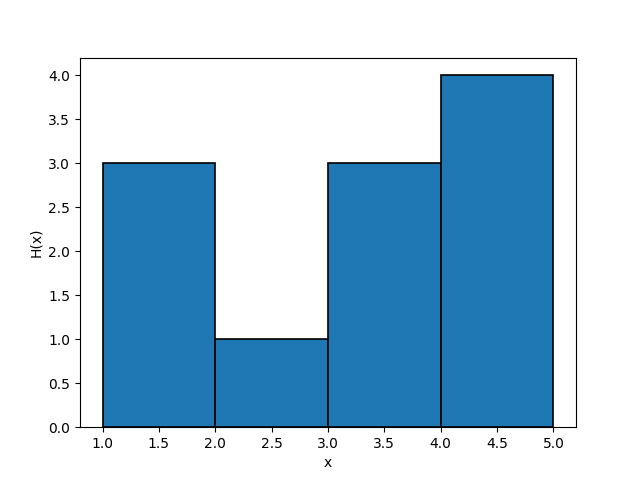
\includegraphics[scale=0.47]{histogram-zgled.png}
        \end{subfigure}
        \begin{subfigure}{0.49\textwidth}
            \centering
            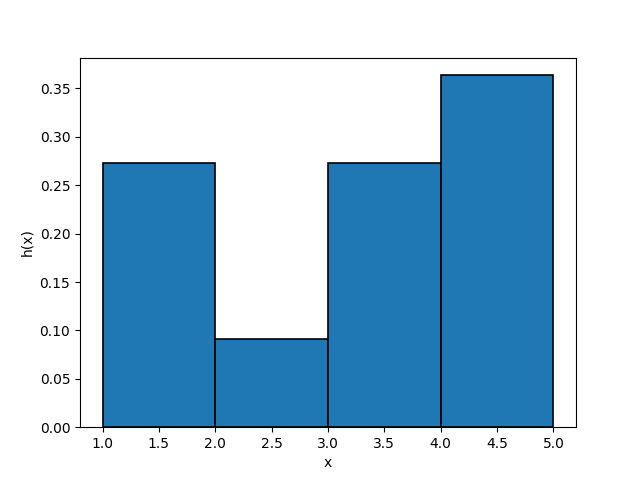
\includegraphics[scale=0.47]{histogram-norm-zgled.png}
        \end{subfigure}
        \caption{Na levi je (navaden) histogram, na desni pa normaliziran histogram vzorca $S_0$. Oblika je ista, razlika je v skali na y-osi.}
        \label{hist-zgled}
    \end{figure}
\end{zgled}

Od zdaj naprej bomo enačili pojma histogram in normaliziran histogram, z obema pa bomo v mislih imeli normaliziran histogram.

V zgledu opazimo, da histogram grafično ni podan kot funkcija. Opišimo  grafičen prikaz histogramov.
